\tikzstyle{arrow} = [thick,->,>=stealth]
\tikzstyle{plain_box} = [rectangle, minimum width=5cm, minimum height=1.2cm, text width=4cm, text centered, draw=black]

\begin{figure}[htb]
    \centering
    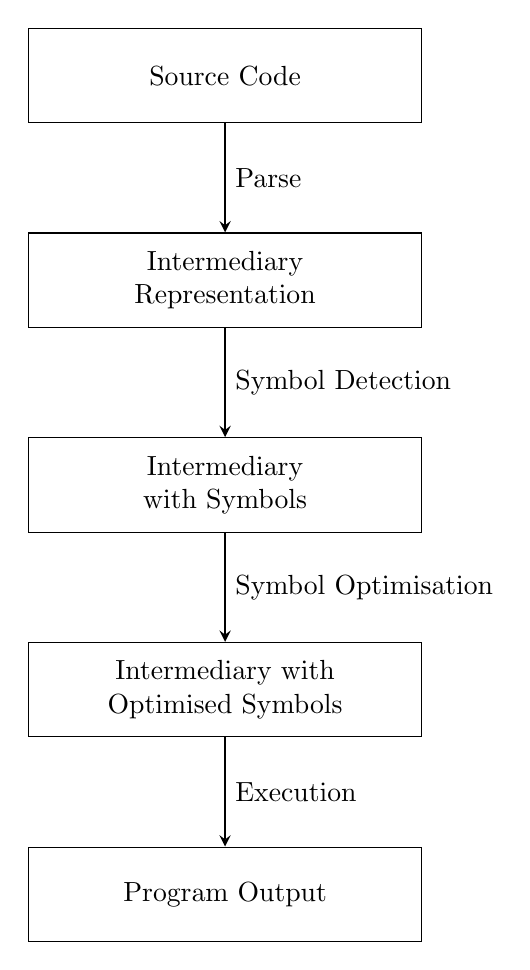
\begin{tikzpicture}[node distance=2.6cm]
        \node (source) [plain_box] {Source Code};
        \node (intermediary) [plain_box, below of=source] {Intermediary Representation};
        \node (intermediary_1) [plain_box, below of=intermediary] {Intermediary with Symbols};
        \node (intermediary_2) [plain_box, below of=intermediary_1] {Intermediary with Optimised Symbols};
        \node (execution) [plain_box, below of=intermediary_2] {Program Output};

        \draw [arrow] (source) -- node[anchor=west] {Parse} (intermediary);
        \draw [arrow] (intermediary) -- node[anchor=west] {Symbol Detection} (intermediary_1);
        \draw [arrow] (intermediary_1) -- node[anchor=west] {Symbol Optimisation} (intermediary_2);
        \draw [arrow] (intermediary_2) -- node[anchor=west] {Execution} (execution);
    \end{tikzpicture}
    \caption{How the Kihi Runner executes a program.}
    \label{fig:kihi_execution_process}
\end{figure}